\section{経路追従モジュール}
\label{sec:imitation}
経路追従モジュールについて述べる.
このモジュールは\ref{chap:path_select}章で述べたシステムに倣って構築した
カメラ画像に基づいて経路を追従するモジュールであり,
分岐路では入力された目標方向に従って経路を選択して走行する.
なお,\ref{chap:path_select}章で述べたシステムに対し,
目標方向とネットワークのパラメータの変更,およびデータセットの
収集手法の追加を行なっている.

% 次に追加した,データセットの収集方法について述べる.
% \ref{chap:path_select}章では,学習器の訓練に60000stepを必要とし,
% 実ロボットを用いた実験に向けて,必要となる学習の量を削減することが望まれる.
% 藤原らが提案する
% データセットに加えるデータの不均衡を改善する手法
% 学習時に積極的に蛇行する手法
% 次に
% \ref{fig:learning_sys}に経路追従モジュールのシステムを示す.


% 学習時は,2D-LiDARやオドメトリ,
% 事前に作成したメトリックマップに基づいた
% ルールベース制御器(ROS Navigation stack)によって,設定した経路を追従する.
% その際,入力をカメラ画像と目標方向,
% 出力をヨー方向の角速度とするデータを,0.2秒周期でデータセットに加える.
% このヨー方向の角速度はメトリックマップに基づいたルールベース制御器が
% 出力する信号である.カメラ画像の収集では
% 中央, 左,右に傾けて取り付けた3つのカメラを用いる.
% 左と右のカメラ画像に対する角速度には,経路に戻るようにオフセットを加える.
% さらに,バッチサイズを8として
% 教師データを抽出し,0.2 秒の周期でオンラインで学習する.
% このデータセットへのデータの追加から学習までの1連の流れを1ステップとする.
% 学習時のデータセットへ加える目標方向には,
% メトリックマップに基づいたルールベースの制御器からの出力を用いる.

% 学習後,モジュールはカメラ画像と目標方向を基に,
% 出力したヨー方向の角速度により経路を追従する.
% このとき,並進速度は 0.2m/s である.
% なお,目標方向が「停止」の場合は,0.0m/s となる.
% \begin{figure}[htbp]
%     \centering
%      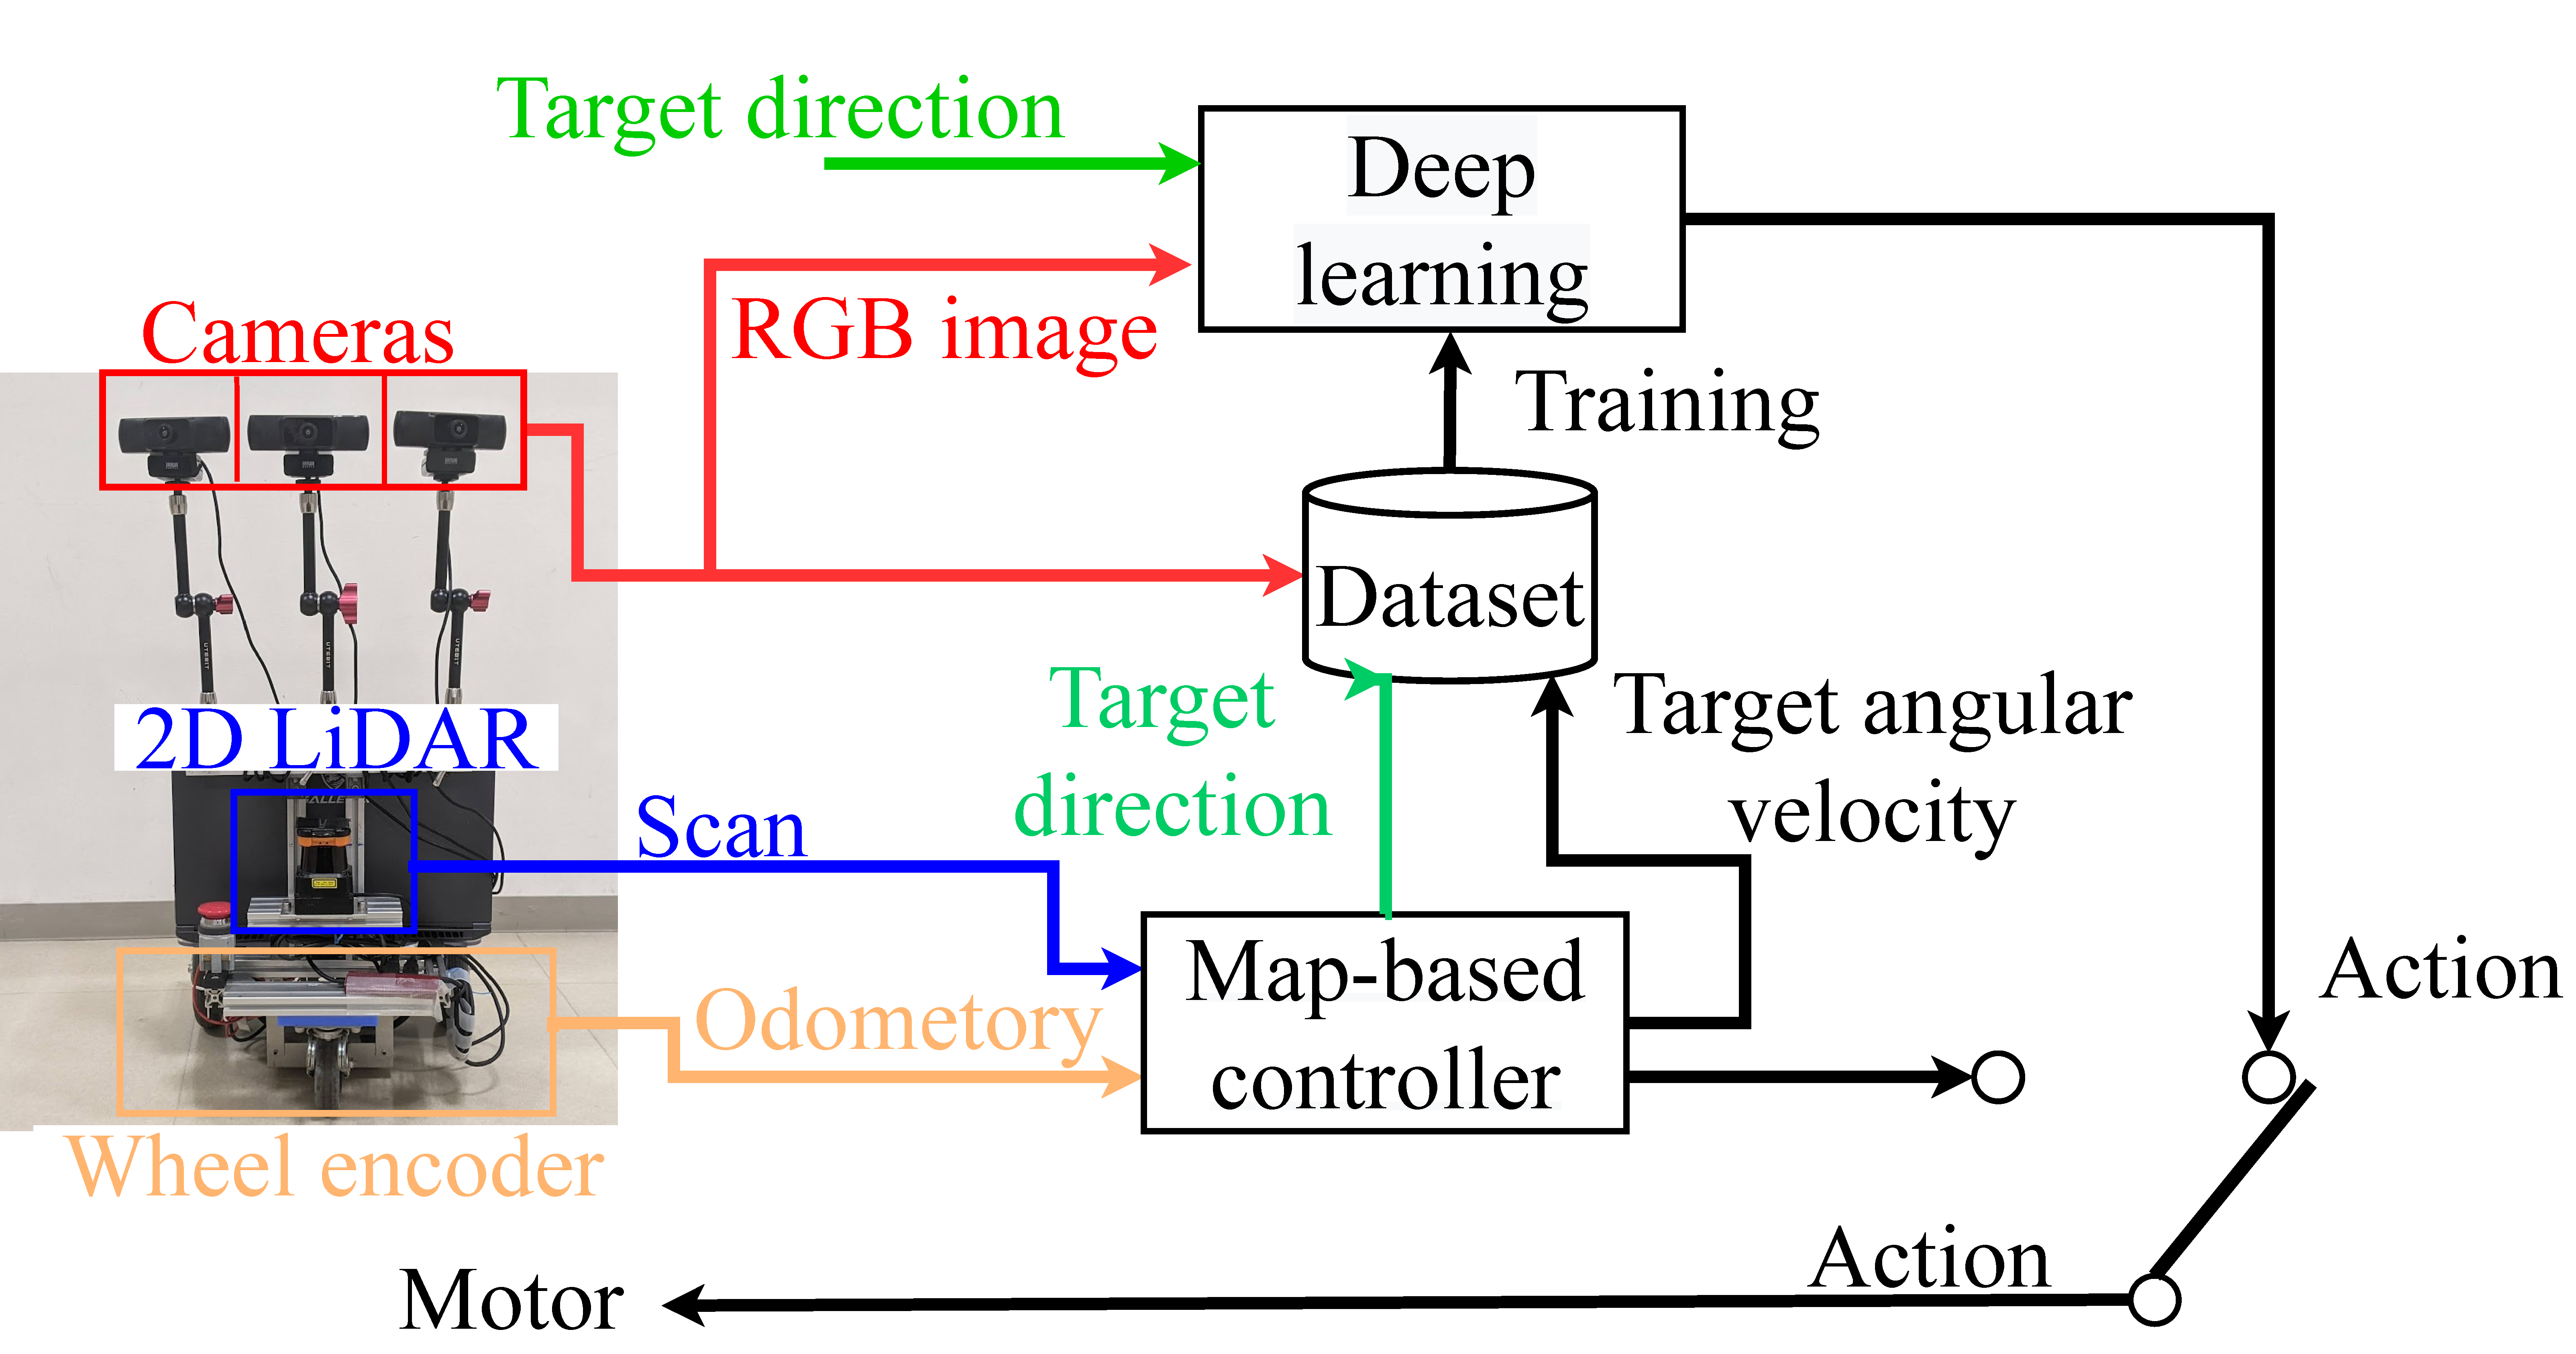
\includegraphics[width=130mm]{images/pdf/system_learning.pdf}
%      \caption{Path-following module system}\label{fig:learning_sys}
% \end{figure}

追加したデータセットの収集手法は,
% % 岡田ら\cite{okada2021}が提案した
% % \begin{quote}
% %     \begin{itemize}
% %      \item 学習器の出力を監視して,経路追従できない場所のデータのみ選択してデータセ
% %      ットに追加する手法
% %     \end{itemize}
% %    \end{quote}
% の他に
学習量の削減を目的に藤原ら\cite{fujiwara2023}が行った以下の2つの手法である.
\begin{quote}
    \begin{itemize}
     \item データセットに加えるデータの不均衡を改善する手法
     \item 学習時に積極的に蛇行する手法
    \end{itemize}
   \end{quote}

データセットに加えるデータの不均衡を改善する手法について述べる.
\figref{fig:oversmple}に,\chapref{chap:path_select}の実験における10000ステップあたりの目標方向
を青で示す.直進のデータが他に比べ圧倒的に多く,不均衡あることが分かる.
Haiboらの調査\cite{hukinko}では,ほとんどの標準的な学習アルゴリズムは,データの不均衡によりパフォー
マンスが大幅に低下するとされている.
そこで,データ前処理手法であるオーバーサンプリングを用いて,データの偏りを改善する.
具体的には,図中赤で示すように左折と右折を7倍に複製する.
\vspace{3zh}
\begin{figure}[htbp]
    \centering
     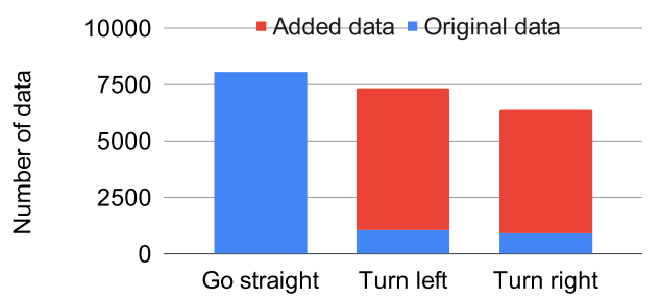
\includegraphics[width=100mm]{images/pdf/oversmple.pdf}
     \caption[Number of data in the target direction per 10000 steps
     in the previous experiment]{Number of data in the target direction per 10000 steps
     in the previous experiment(Quoted from \cite{fujiwara2023})}\label{fig:oversmple}
\end{figure}
\clearpage
次に,学習時に積極的に蛇行する手法について述べる.
学習時に経路から離れた状態が増加すると,訓練済みの学習器での走行時に経路から
外れることが減少し,より少ない学習時間で成功率が高いモデルが獲得できる可能性がある.
そのため,学習時に積極的に蛇行する手法では\figref{fig:dakou}に示すように,
学習時のロボットの制御に用いるヨー方向の角速度を1.5倍にする.
これにより,大きく蛇行して,目標経路から離れた状態を多く収集する.
\vspace{3zh}
\begin{figure}[htbp]
    \centering
     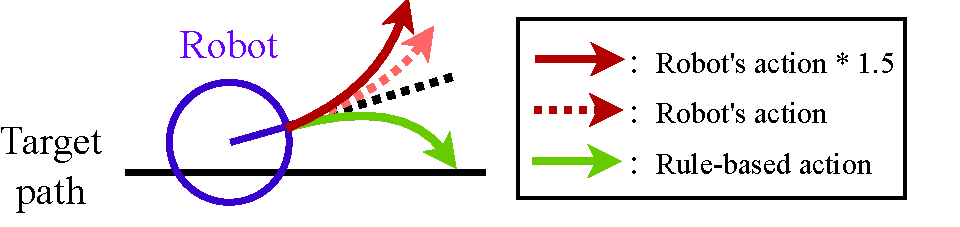
\includegraphics[width=130mm]{images/pdf/dakou.pdf}
     \caption[Aggressive meandering]{Aggressive meandering(Quoted from \cite{fujiwara2023})}\label{fig:dakou}
\end{figure}
藤原らは実験により,これらの2つのデータセットの収集手法によって,
経路追従の成功率を下げること無く,必要な学習量を60000ステップから
20000ステップまで削減できることを確認している.
\newpage

\tabref{tab:target}に変更した目標方向とそのデータ形式を示す.
\chapref{chap:path_select}における
目標方向の中で,ContinueとGo straightは同じ方向を指しているため,本章ではこれらを1つとして扱う.
これに伴い,ワンショットベクトルの次元数を4から3へ変更している.
さらに,目的地に到着後,ロボットを停止させることを目的として,
Stop(停止)の目標方向を追加した.
停止の目標方向が入力された際は,ロボットの並進速度は0.0m/sとなり,ロボットはその場で停止する.
% なお,停止以外の目標方向における並進速度は\chapref{chap:path_select}と同様に0.2m/sである.
% 「停止」が入力された場合は0.0m/sとなる.

目標方向の次元数の変更に伴い,修正を加えたネットワークの構造を\figref{fig:imi_net}に示す.
具体的には,CNNの出力と目標方向を入力する全結合層の入力サイズを260から259へ調整している.

\begin{table}[htbp]
    \centering
    \caption{Target direction and data for path-following module}\label{tab:target}
    \begin{tabular}{|c|c|}
    \hline
    Target direction & Data        \\
    \hline
    Go straight   & {[}1,0,0{]} \\
    Turn left   & {[}0,1,0{]} \\
    Turn right   & {[}0,0,1{]} \\
    Stop   & {[}0,0,0{]}\\
    \hline
    \end{tabular}
    \end{table}
% 経路追従モジュールで用いるネットワークの構造を\ref{fig:imi_net}に示す.
% ネットワークはRGB画像と,目標方向を入力,ヨー方向の角速度を出力として
% end-to-endで学習する.
% ネットワークは,画像を処理するCNNアーキテクチャ,
% CNNの出力と目標方向を入力とする全結合層で構成されている.
\begin{figure}[htbp]
    \centering
     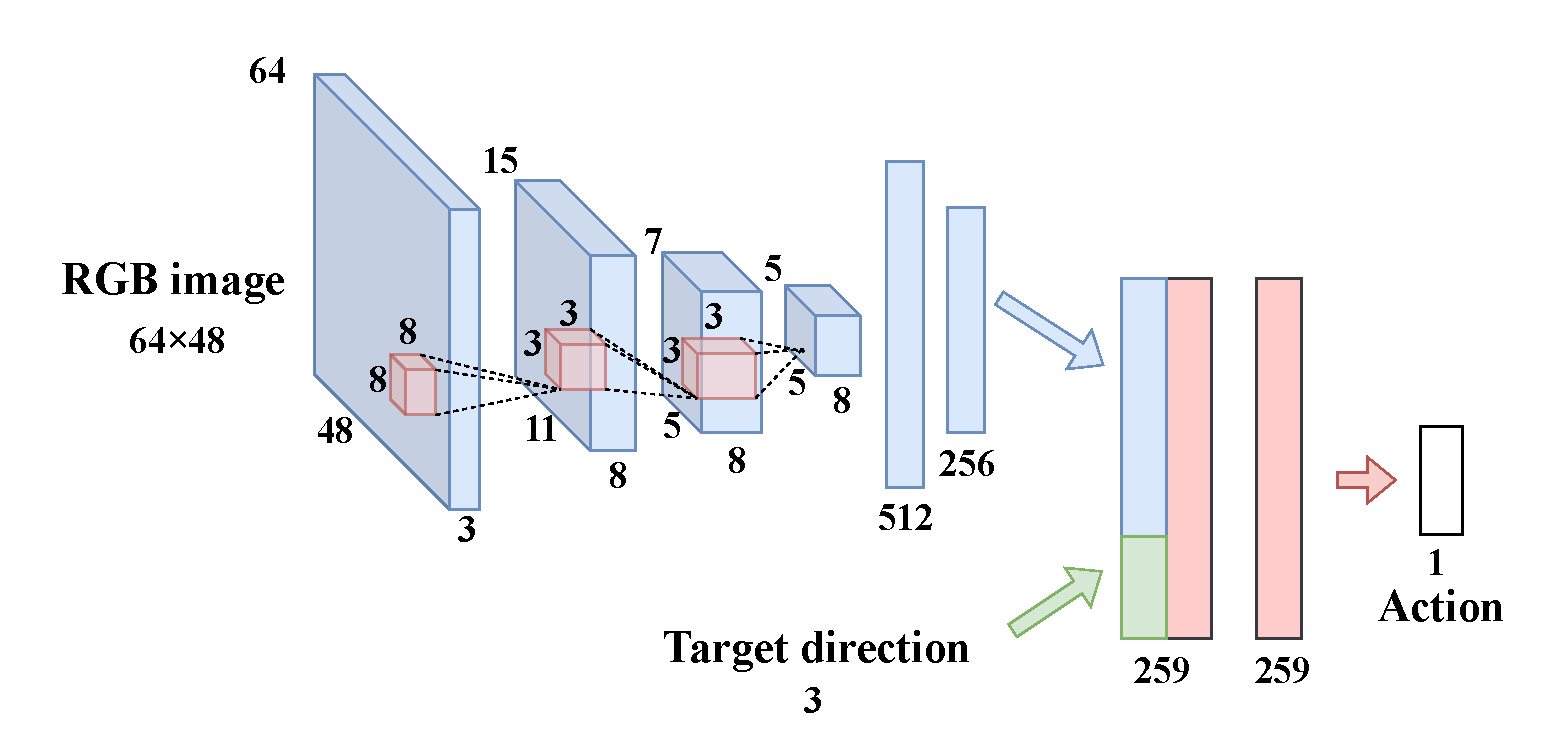
\includegraphics[width=130mm]{images/pdf/imi_net.pdf}
     \caption{Structure of the network of path-following module}
     \label{fig:imi_net}
\end{figure}

% 目標方向は\ref{tab:target}に示す
% 直進,左折,右折の3つをワンホットベクトルとして入力する.
% この中で,停止はネットワークへは入力せず,
% この目標方向が停止の場合には,前述の通り並進速度,角速度ともに0.0m/sとする.
